%================================================================
\section{Theory}\label{sec:Theory}
%================================================================

%----------------------------------------------------------------
\subsection{Project Theory 1}\label{sec:project theory}
%----------------------------------------------------------------
This is \autoref{sec:project theory}.

Citation is done with \hologo{BibTeX} \cite[p.~100]{Sakurai}.

Cross-reference equations such as
\begin{equation}\label{eq:einstein}
    E = m c^2
\end{equation}
with \cref{eq:einstein}.

\autoref{fig:noise} brings the noise from the \textbf{figures folder}. 
\begin{figure}[H]
\begin{center}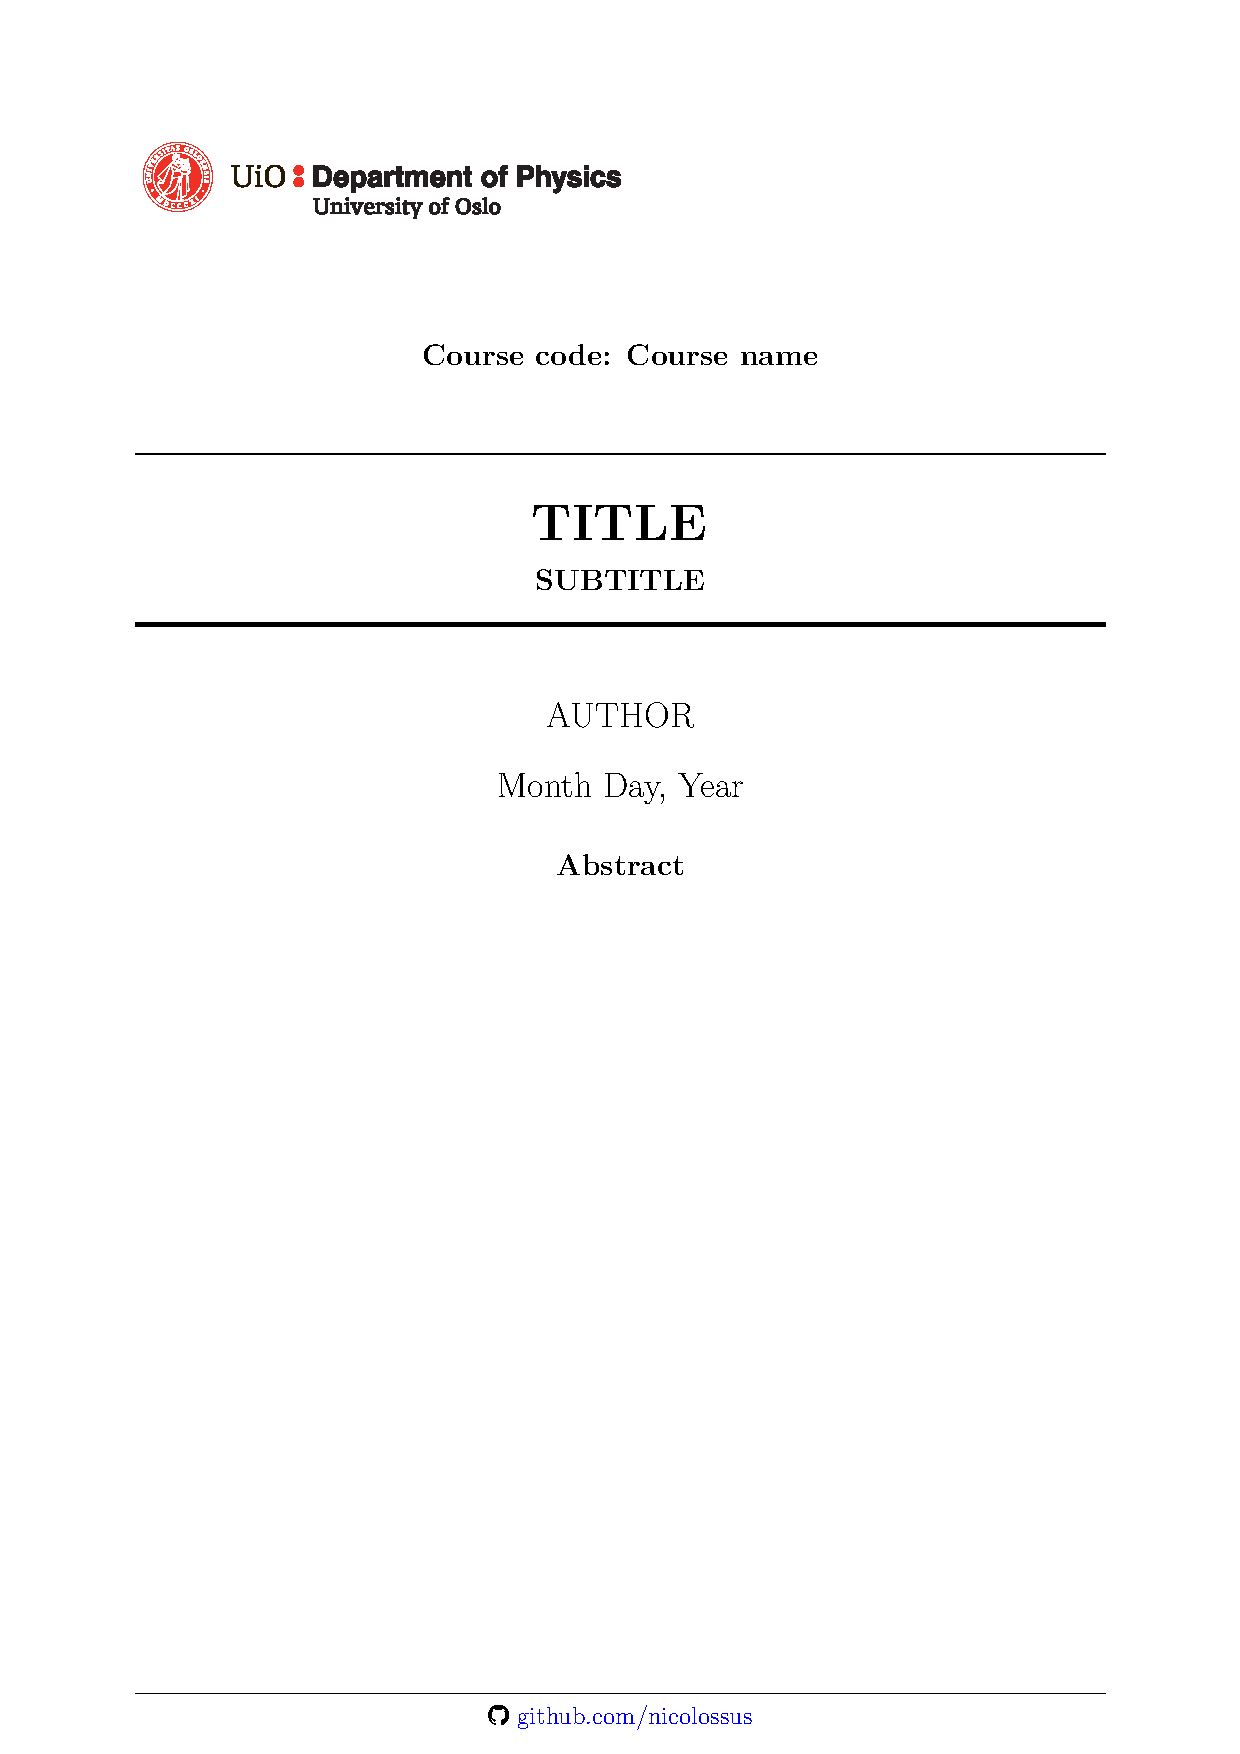
\includegraphics[scale=0.5]{example} 
\end{center}
\caption{Make some noise.}
\label{fig:noise}
\end{figure}

\autoref{fig:happy} shows a happy animal found in the \textbf{Images folder}. 
\begin{figure}[H]
\begin{center}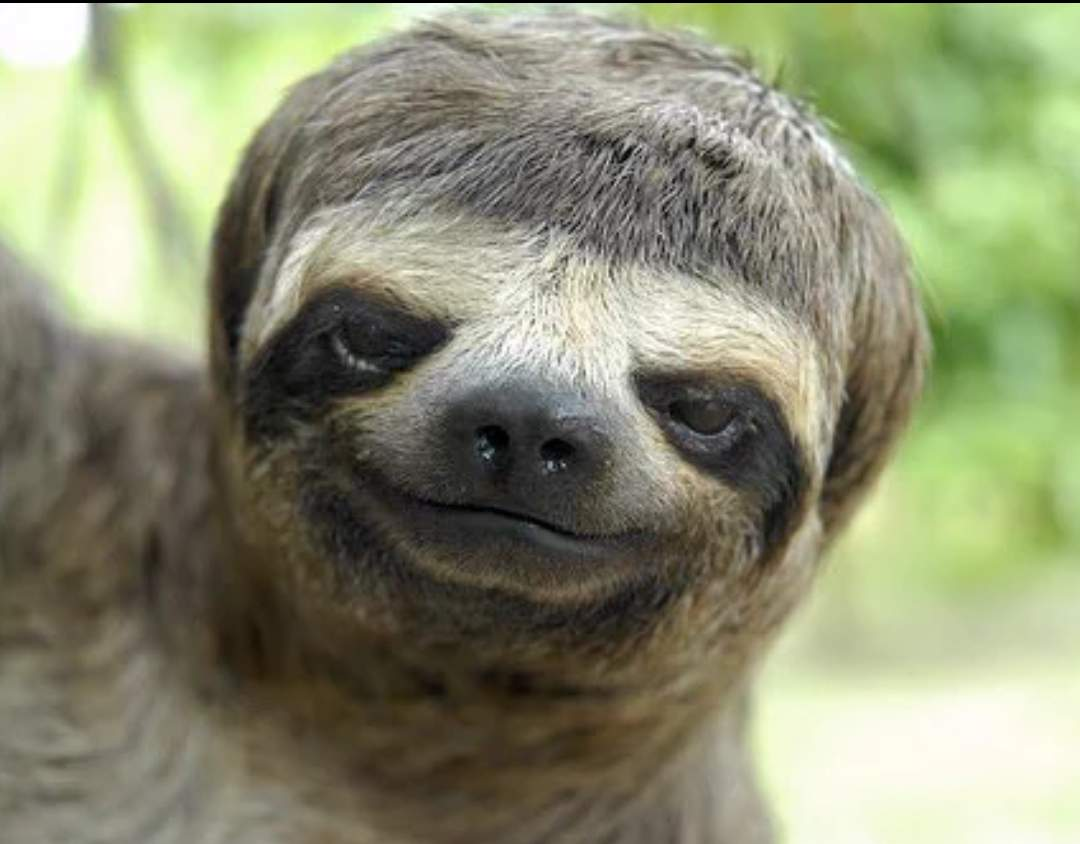
\includegraphics[scale=0.5]{./Images/Funny-Animal-Face} 
\end{center}
\caption{Sloths are arboreal mammals noted for slowness of movement and for spending most of their lives hanging upside down in the trees.}
\label{fig:happy}
\end{figure}

\autoref{tab:tab1} is from the \textbf{tables folder}. 
\begin{table}[H]
\caption{From pandas to latex.}
\centering
\rowcolors{2}{gray!25}{white}
\begin{tabular}{ccc}
\hline \hline
  $x$ &  $x^2$ &  $x^3$ \\
\hline \hline
0.250 &  0.062 &  0.016 \\
0.500 &  0.250 &  0.125 \\
0.750 &  0.562 &  0.422 \\
\hline \hline
\end{tabular}

\label{tab:tab1}
\end{table}

\autoref{tab:alternate} tabulates some values with alternating row colors.
\begin{table}[H]
\caption{Alternating background color for rows.}
\centering
\rowcolors{2}{gray!25}{white}
\begin{tabular}{ccc}
\hline
\hline 
$\alpha$ & $\beta$ & $\gamma$
\\
\hline 
\hline 
0.1 & 0.2 & 0.3
\\
0.4 & 0.5 & 0.6
\\
0.7 & 0.8 & 0.9
\\
\hline
\hline 
\end{tabular}
\label{tab:alternate}
\end{table}

Given
\begin{align*}
    f\colon \R \to \R,
    \intertext{magic happens}
    \int_{0}^{\infty} \mathrm{e}^{-x}\,\mathrm{d}x
\end{align*}
